\documentclass[11pt, oneside]{article}   	% use "amsart" instead of "article" for AMSLaTeX format
%\usepackage{geometry}                		% See geometry.pdf to learn the layout options. There are lots.
%\geometry{letterpaper}                   		% ... or a4paper or a5paper or ... 
%\geometry{landscape}                		% Activate for rotated page geometry
%\usepackage[parfill]{parskip}    		% Activate to begin paragraphs with an empty line rather than an indent

\usepackage{geometry}
 \geometry{
 a4paper,
 total={170mm,257mm},
 left=20mm,
 top=25mm,
 bottom=25mm
 }

\usepackage{graphicx}				% Use pdf, png, jpg, or eps§ with pdflatex; use eps in DVI mode
								% TeX will automatically convert eps --> pdf in pdflatex		
\usepackage{amssymb}
\usepackage{amsmath}
\usepackage{fancyhdr}
\usepackage[utf8]{inputenc}
\usepackage[english]{babel}
\usepackage{enumerate}
\usepackage{arcs}
\usepackage{cancel}
\usepackage{xfrac}
\usepackage{amsthm}
\usepackage{gensymb}
\usepackage{xspace}
%\usepackage{ctex}
\usepackage{subcaption}

%SetFonts

%SetFonts

\usepackage[inline]{asymptote}


\pagestyle{fancy}
\fancyhf{}
\rhead{David (Zifei) Zhong, zhongz@email.sc.edu}
\lhead{\leftmark}
%\lfoot{Copyright \copyright 2021-2022 by Teacher David. All rights reserved.}

\title{CSCE 790, Report for Project 1}
\author{Zifei (David) Zhong}
\date{February 21, 2023}							% Activate to display a given date or no date

\newcommand{\latex}{\LaTeX\xspace}


\begin{document}
\maketitle

This report is consist of two parts: 1) part one provides analysis over 6 audio recordings with different sample rates; 2) part two provides a method to separate an audio into small chunks, each of which corresponds to a letter spoken in the audio.

\section{Part One: Sample Audio Signals}
In this experiment, I recorded 6 audios. For each audio recording, I only spoke the three letters `U', `S', and `C' with a clear separation in time. Each audio recording lasted for 5 seconds.

Figure~\ref{fig:amplitude} shows the amplitude of audios with sampling rates 8k Hz, 16k Hz, 24k Hz, 32k Hz, 40k Hz, and 48k Hz. The amplitudes of each recording are almost the same, with little difference, since the audios were spoken the same person (me) with similar tones. The only difference is that the number of samples for each audio file increases as the sampling frequency increases. The number of samples can be calculated by $$ \text{\# of samples} = \text{sample\_rate (Hz)} \times \text{sample\_time (s)}.$$ 

For example, in Figure~\ref{fig:amplitude}(f), with 48k Hz sample rate, the 5 second audio results $48000 \times 5 = 240,000$ samples, as indicated in the horizontal axis of the figure.

\begin{figure}[ht]
\centering
\begin{subfigure}[b]{0.3\textwidth}
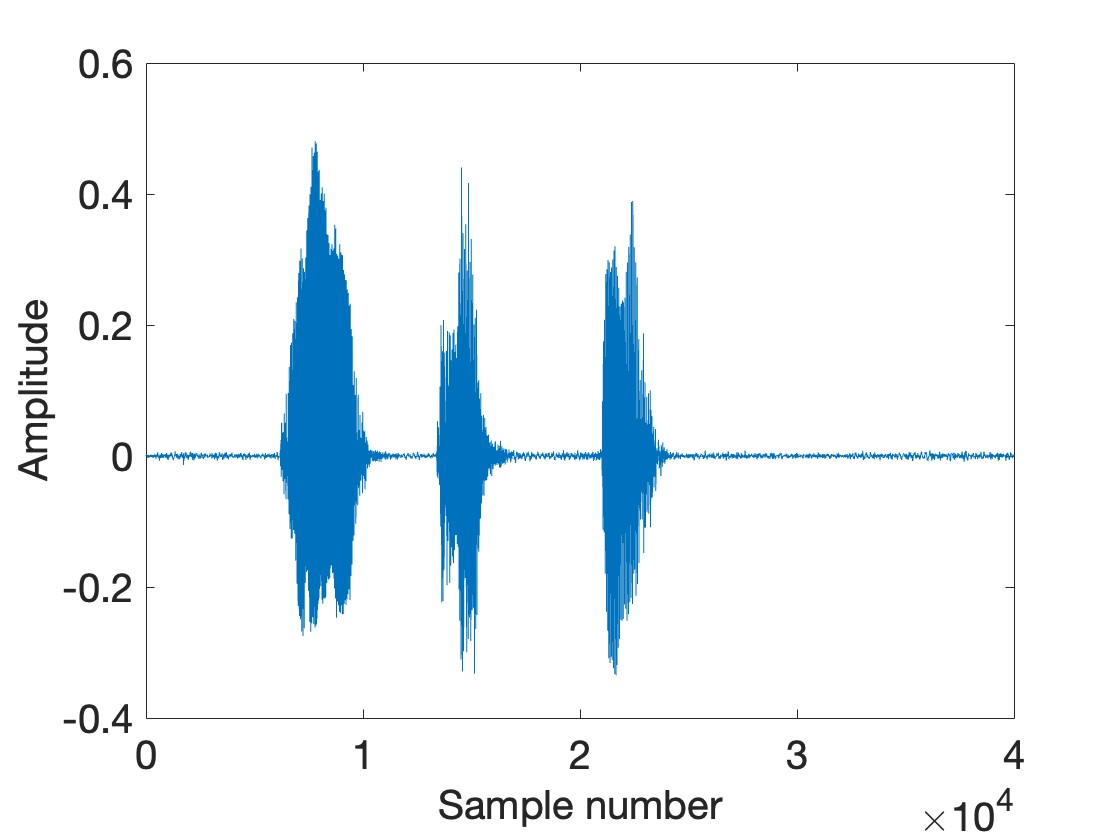
\includegraphics[width=\textwidth]{imgs/8k-amplitude.jpg}
\caption{8k Hz}
\end{subfigure}
\begin{subfigure}[b]{0.3\textwidth}
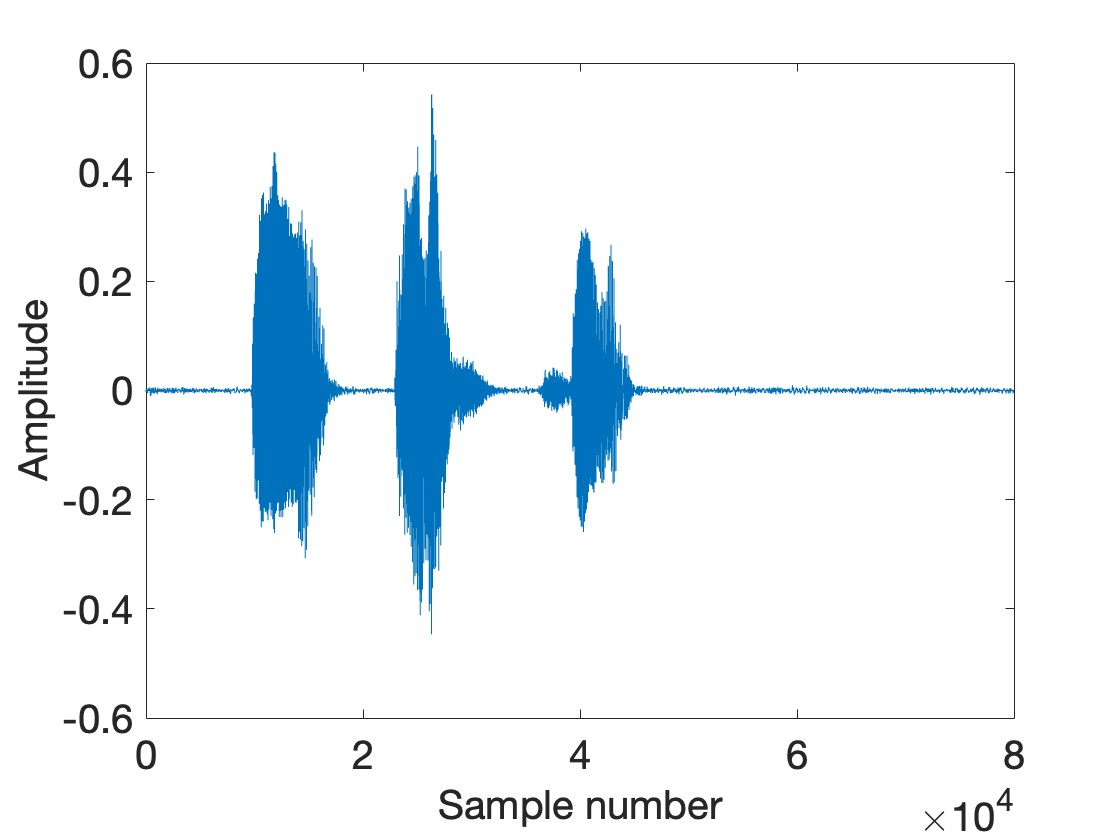
\includegraphics[width=\textwidth]{imgs/16k-amplitude.jpg}
\caption{16k Hz}
\end{subfigure}
\begin{subfigure}[b]{0.3\textwidth}
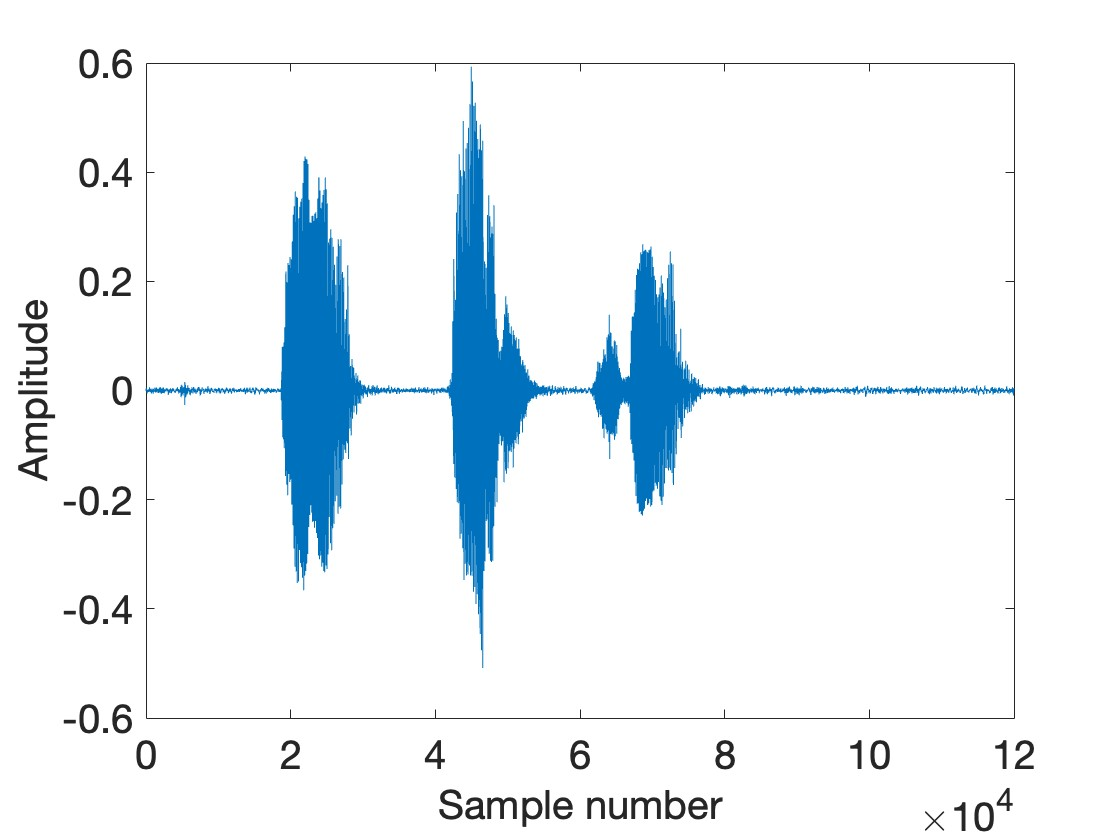
\includegraphics[width=\textwidth]{imgs/24k-amplitude.jpg}
\caption{24k Hz}
\end{subfigure}\\
\begin{subfigure}[b]{0.3\textwidth}
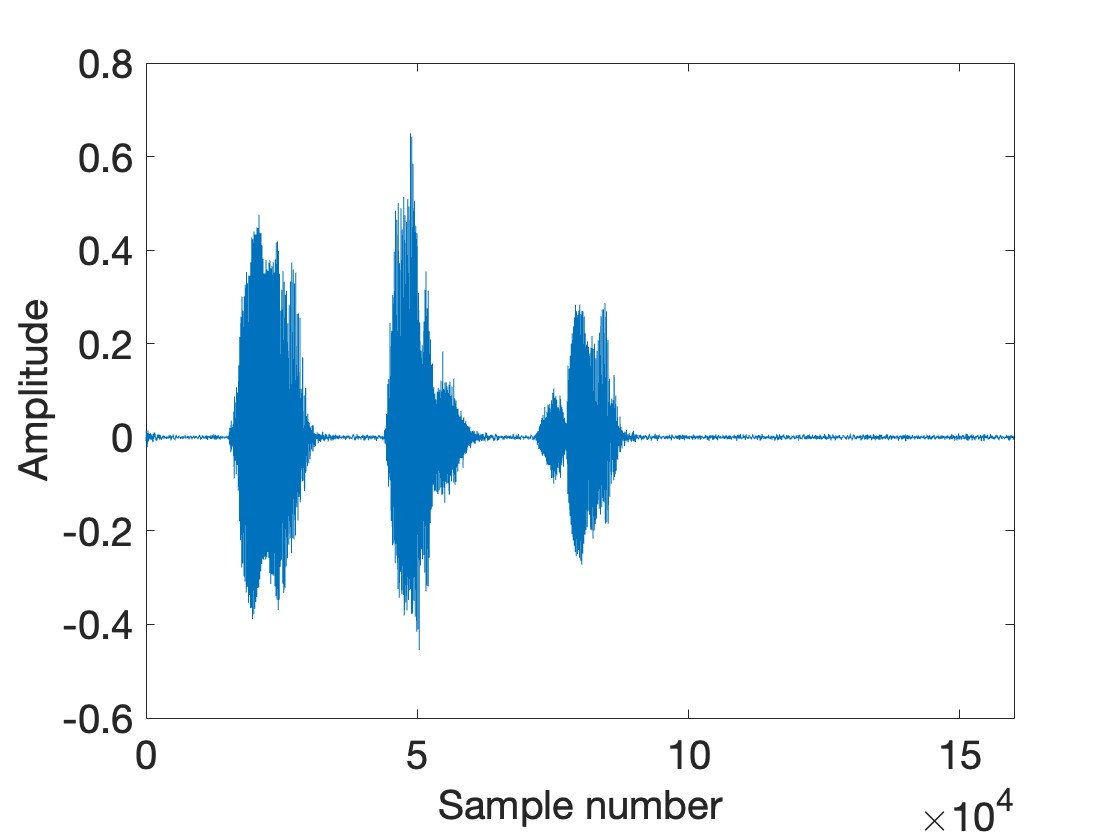
\includegraphics[width=\textwidth]{imgs/32k-amplitude.jpg}
\caption{32k Hz}
\end{subfigure}
\begin{subfigure}[b]{0.3\textwidth}
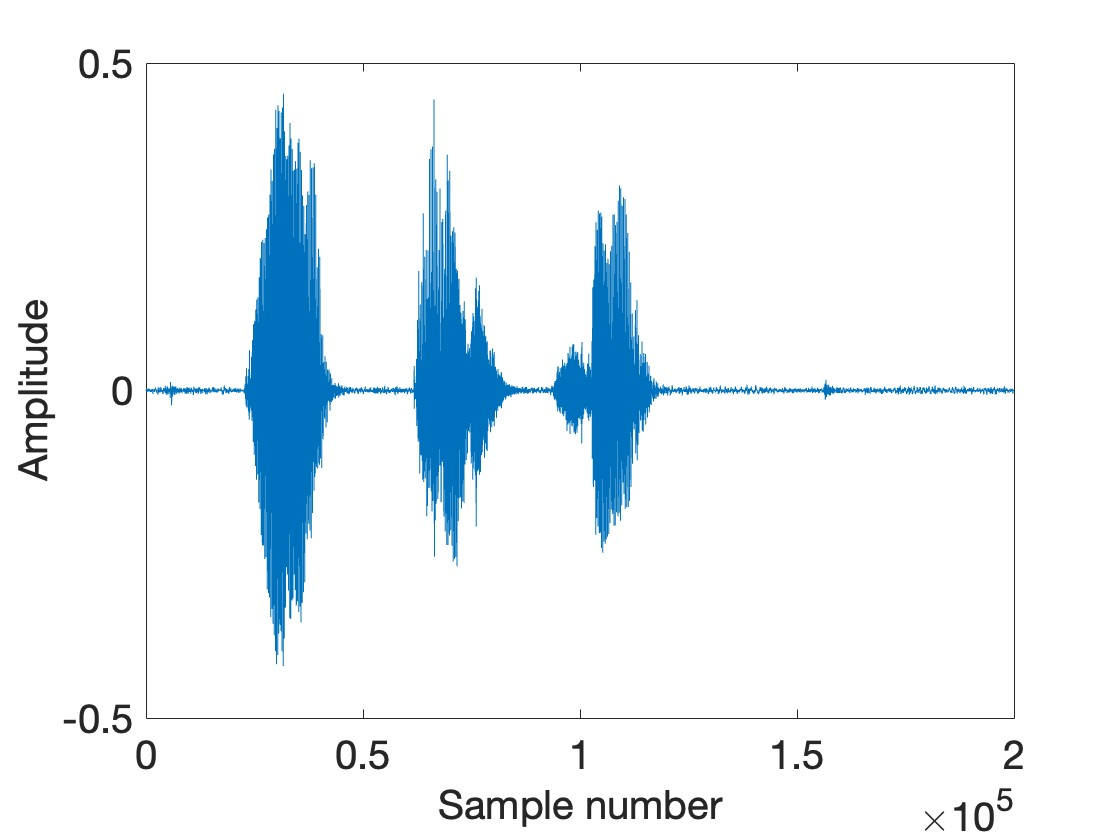
\includegraphics[width=\textwidth]{imgs/40k-amplitude.jpg}
\caption{40k Hz}
\end{subfigure}
\begin{subfigure}[b]{0.3\textwidth}
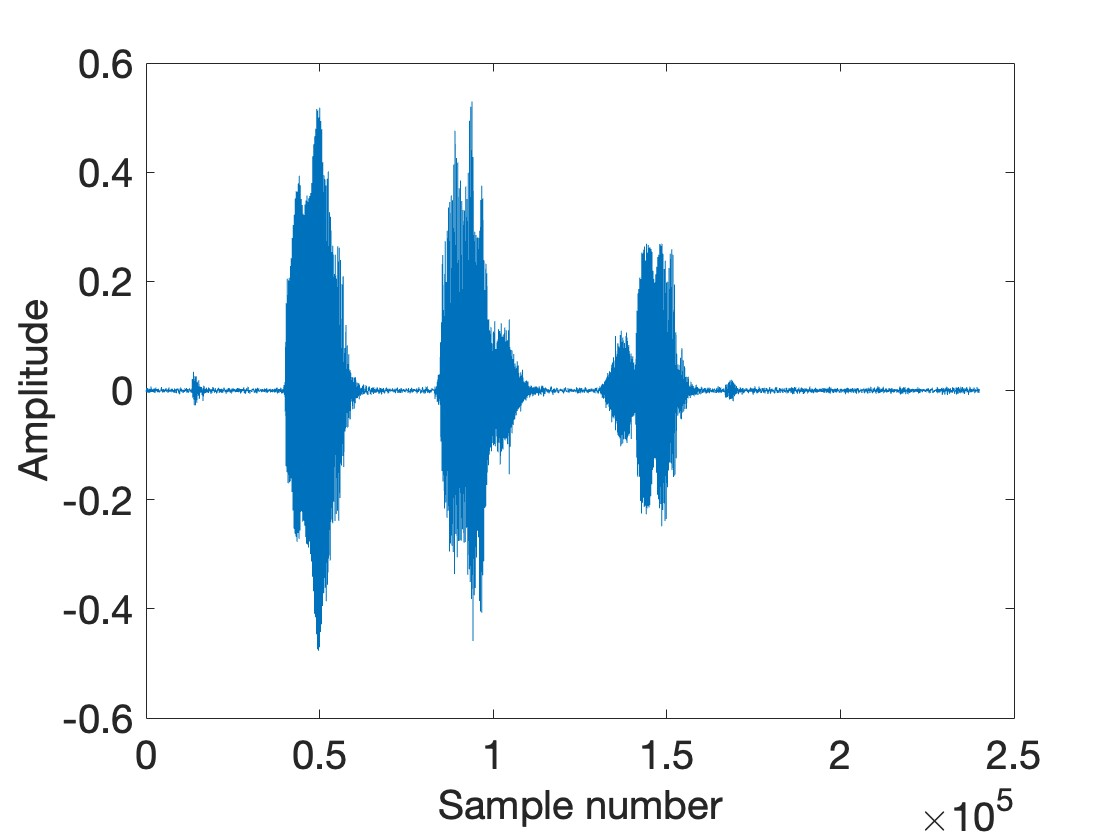
\includegraphics[width=\textwidth]{imgs/48k-amplitude.jpg}
\caption{48k Hz}
\end{subfigure}

\caption{Amplitude of audios with different sampling rates}
\label{fig:amplitude}
\end{figure}

Figure~\ref{fig:spectrogram} shows the spectrogram of audios with sampling rates 8k Hz, 16k Hz, 24k Hz, 32k Hz, 40k Hz, and 48k Hz. The power levels for all figures are all between $-140$dB to $-40$dB. Again, this is because the audios are generated by the same person with similar tones. We should notice that different sample rates result difference in the maximum frequencies that were captured. Since the \emph{Nyquist rate} for sampling a signal with maximum frequency $f$ is $2f$, in our experiment with a 8k Hz sampling rate we can only capture signals with frequency less than 4k Hz. Signals with frequency higher or equal to 8k Hz will be aliased. 

With higher sampling rate, we can correctly capture signals that has higher frequency without aliasing. From Figure~\ref{fig:spectrogram} we can see that when the sampling rate reaches 32k Hz, the frequencies with high power level are mainly stay below 16k Hz. This means that with a sampling rate about 32k Hz, the recorded audios should have captured corresponding human speaking with good quality.

\begin{figure}[ht]
\centering
\begin{subfigure}[b]{0.3\textwidth}
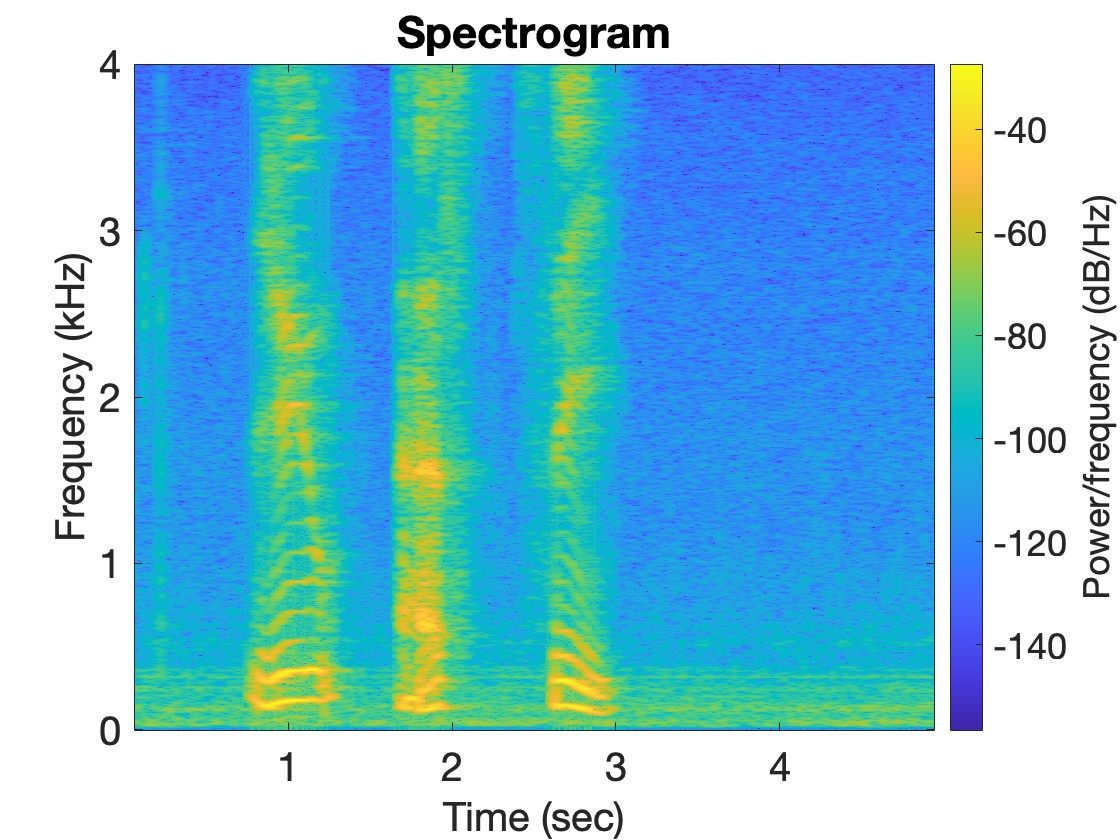
\includegraphics[width=\textwidth]{imgs/8k-spectrogram.jpg}
\caption{8k Hz}
\end{subfigure}
\begin{subfigure}[b]{0.3\textwidth}
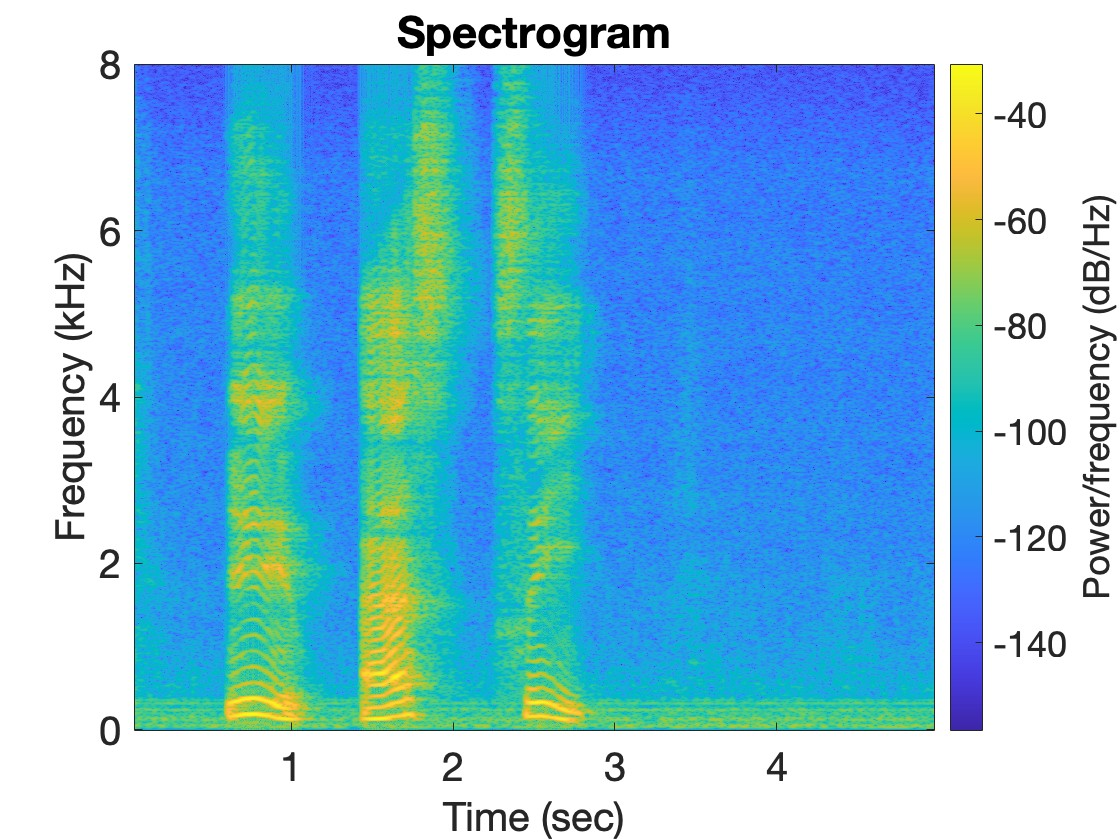
\includegraphics[width=\textwidth]{imgs/16k-spectrogram.jpg}
\caption{16k Hz}
\end{subfigure}
\begin{subfigure}[b]{0.3\textwidth}
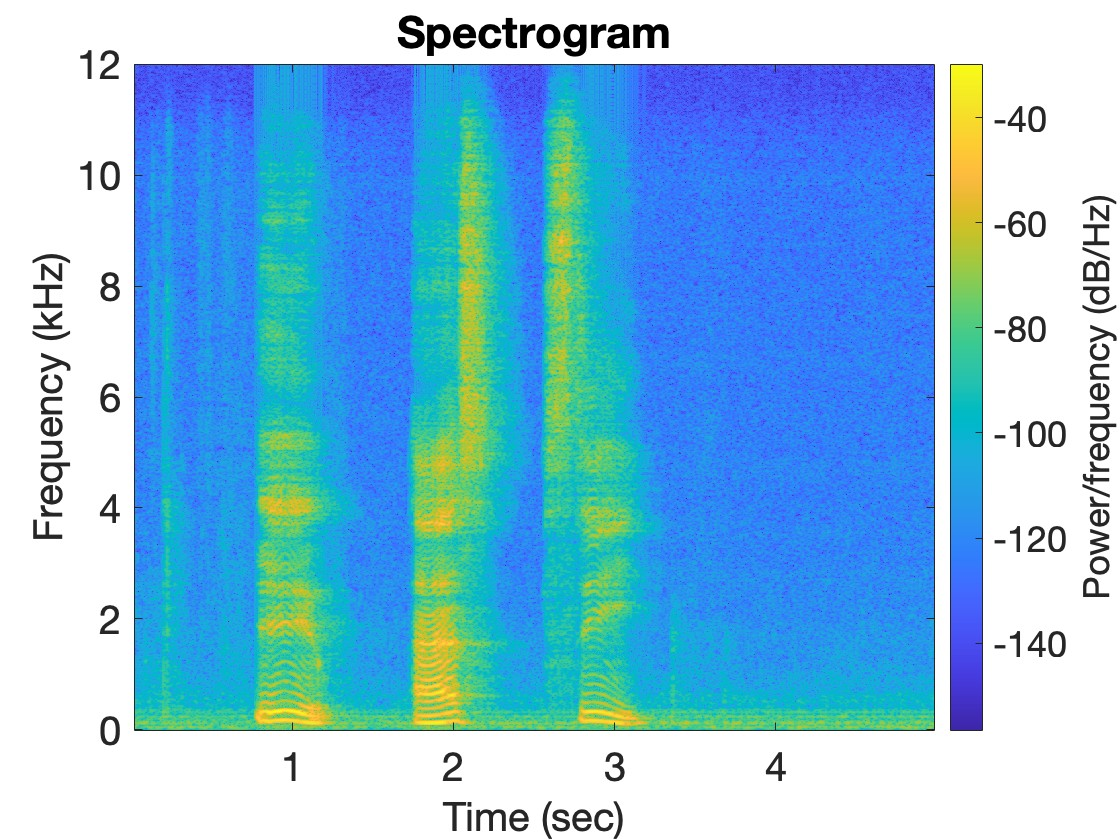
\includegraphics[width=\textwidth]{imgs/24k-spectrogram.jpg}
\caption{24k Hz}
\end{subfigure}\\
\begin{subfigure}[b]{0.3\textwidth}
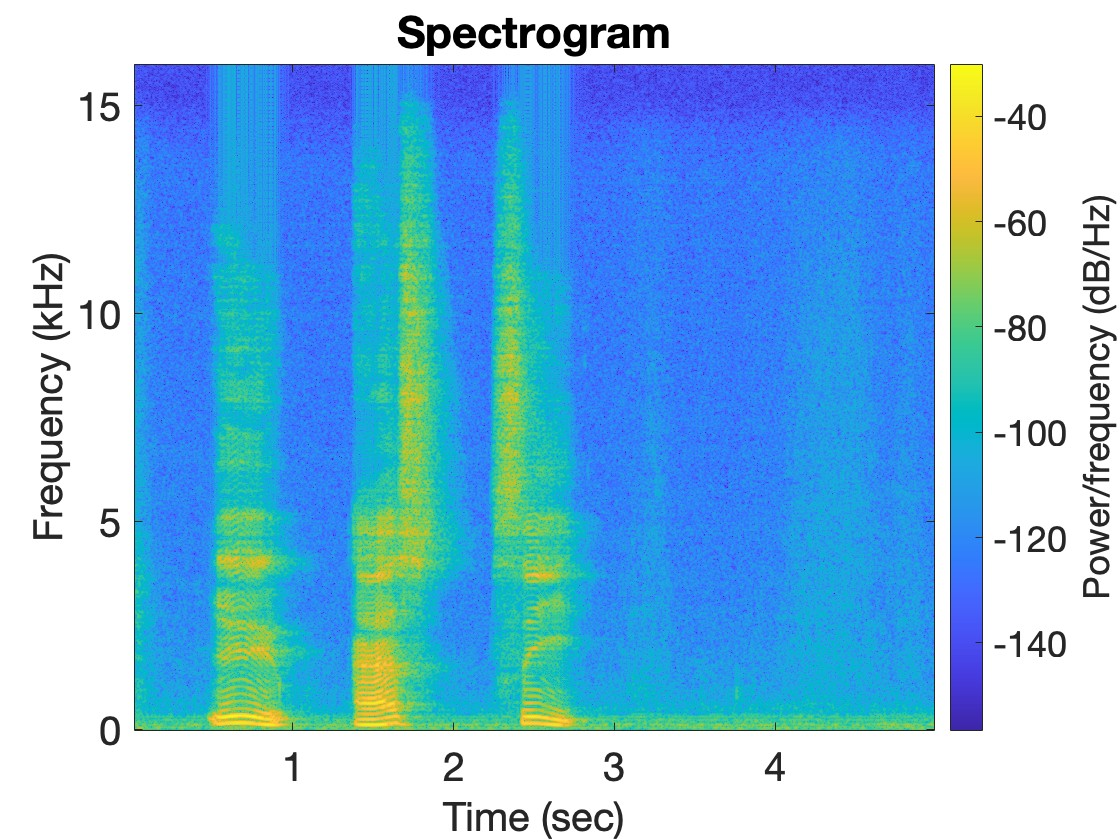
\includegraphics[width=\textwidth]{imgs/32k-spectrogram.jpg}
\caption{32k Hz}
\end{subfigure}
\begin{subfigure}[b]{0.3\textwidth}
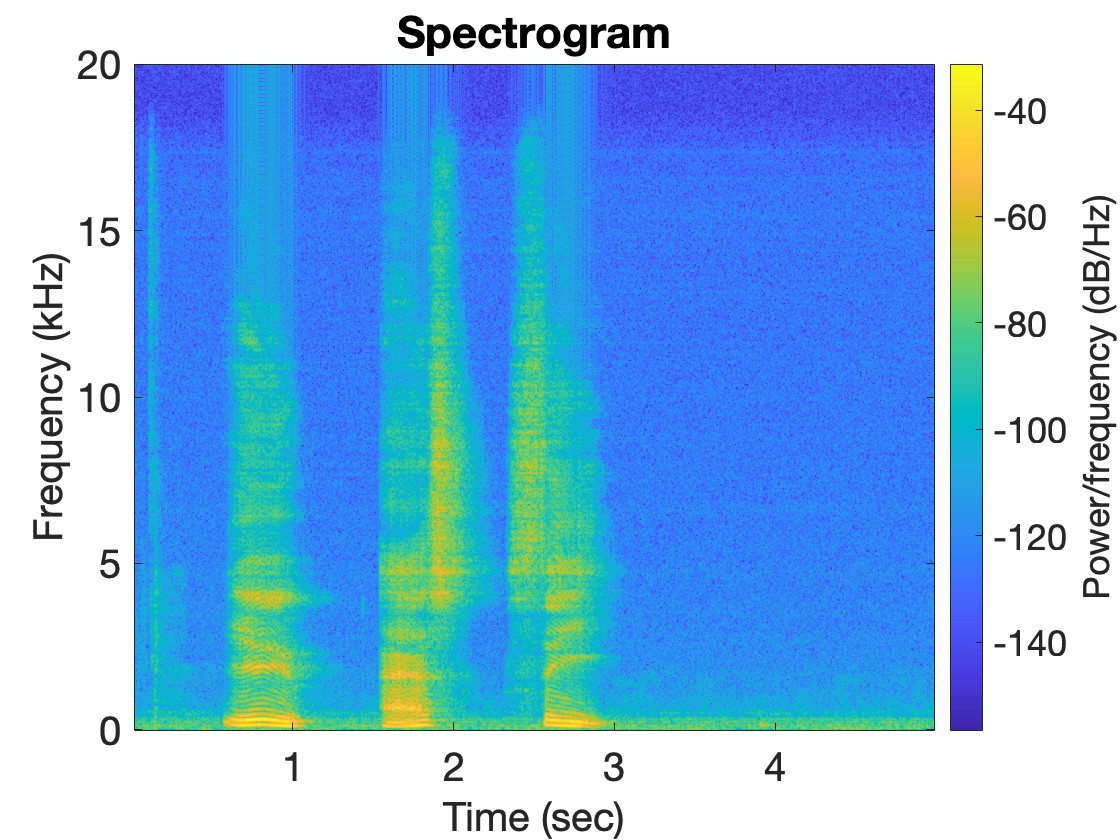
\includegraphics[width=\textwidth]{imgs/40k-spectrogram.jpg}
\caption{40k Hz}
\end{subfigure}
\begin{subfigure}[b]{0.3\textwidth}
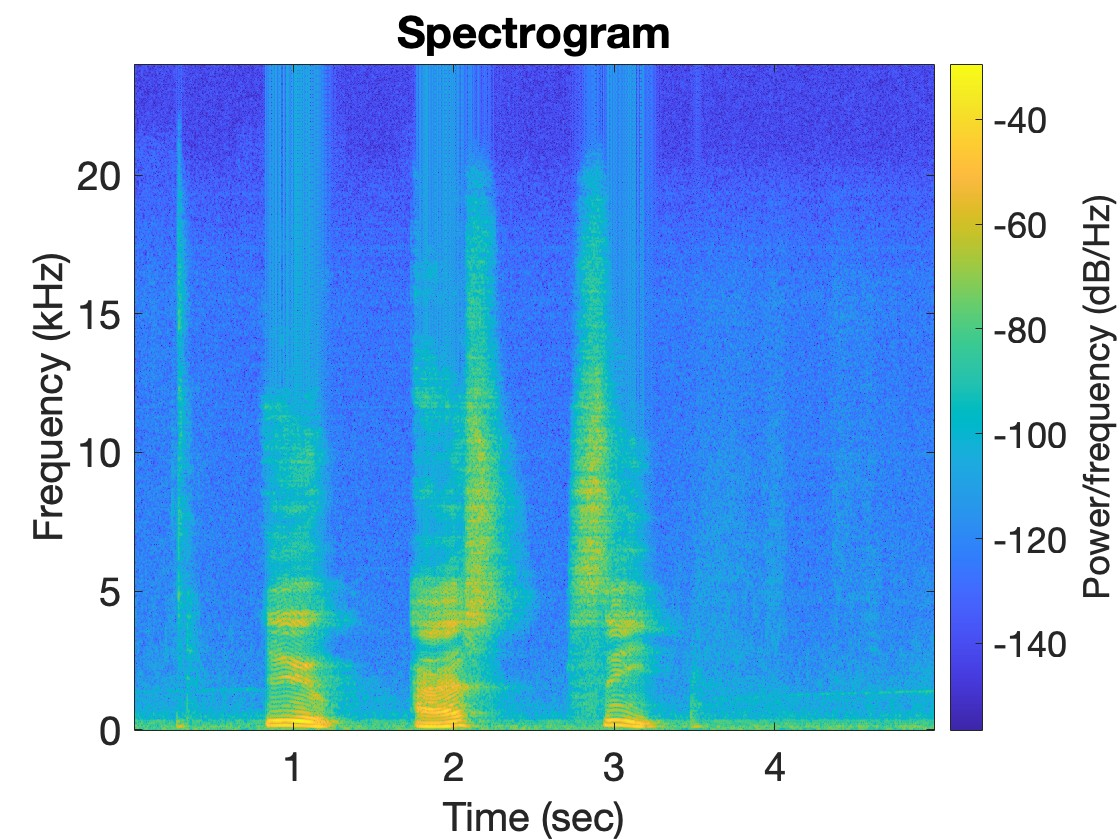
\includegraphics[width=\textwidth]{imgs/48k-spectrogram.jpg}
\caption{48k Hz}
\end{subfigure}

\caption{Spectrogram of audios with different sampling rates}
\label{fig:spectrogram}
\end{figure}

Overall, Table~\ref{tab:compare} compares the characteristics of all 6 audio files. As the sampling rate increases, the number of samples increases proportionally, and the size of the file increases proportionally as well. When the sampling rate is 8k Hz, the audio file is muffled (low quality). When sampling rate reaches 32k Hz, the audio file quality is very good with no obvious muffling. Obviously, the maximum frequency captured by each audio file increases proportionally to the sampling rate.

\begin{table}[ht]
\centering
\caption{Characteristics of different audio samples}
\label{tab:compare}
\begin{tabular}{|c|c|c|c|c|c|c|}
\hline
Audio File & Duration & Sampling Rate & \# Samples & File Size (k) & Quality & Max Freq\\
\hline
\hline
8k\_audio.wav & 5 s & 8k Hz & 40,000  & 78 & muffled & 4k Hz\\
16k\_audio.wav & 5 s & 16k Hz & 80,000  & 78 & clear & 8k Hz\\
24k\_audio.wav & 5 s & 24k Hz & 120,000  & 156 & clear & 12k Hz\\
32k\_audio.wav & 5 s & 32k Hz & 160,000  & 234 & very clear & 16k Hz\\
40k\_audio.wav & 5 s & 40k Hz & 200,000  & 313 & very clear & 20k Hz\\
48k\_audio.wav & 5 s & 48k Hz & 240,000  & 391 & very clear & 24k Hz\\
\hline
\end{tabular}
\end{table}


\end{document} 